\documentclass[12pt]{article}

\usepackage[a4paper,margin=2.5cm]{geometry}
\usepackage{amsmath, amssymb, amsthm}
\usepackage{bm}
\usepackage{hyperref}
\usepackage{graphicx}
\usepackage{caption}
\usepackage{listings}
\usepackage{xcolor}
\usepackage{float}
\usepackage{placeins}
\graphicspath{{figures/}}

\lstdefinestyle{code}{
  basicstyle=\ttfamily\small,
  numbers=left,
  numberstyle=\tiny,
  numbersep=8pt,
  keywordstyle=\color{blue},
  commentstyle=\color{teal!70!black},
  stringstyle=\color{orange!70!black},
  showstringspaces=false,
  breaklines=true,
  frame=single,
  framerule=0.3pt,
  rulecolor=\color{black!15}
}
\lstset{style=code}

\title{t-SNE Tutorial}
\author{}
\date{\today}

\begin{document}
\maketitle

\section{Introduction}
t-Distributed Stochastic Neighbor Embedding (t-SNE) is a non-linear dimensionality reduction technique for visualizing high-dimensional data in two or three dimensions. It converts pairwise distances into probabilities and minimizes the Kullback--Leibler (KL) divergence between neighborhoods in the original and embedded spaces, yielding intuitive visual clusters.

\section{Theory and Formulas}
\subsection{Pairwise Similarities}
For high-dimensional points \(\mathbf{x}_i\), t-SNE defines conditional probabilities that measure neighbor affinity:
\begin{equation}
p_{j|i} = \frac{\exp\left(-\lVert \mathbf{x}_i - \mathbf{x}_j \rVert_2^2 / 2\sigma_i^2\right)}{\sum_{k \neq i} \exp\left(-\lVert \mathbf{x}_i - \mathbf{x}_k \rVert_2^2 / 2\sigma_i^2\right)},
\end{equation}
where \(\sigma_i\) is set so that the perplexity of the distribution equals a user-specified value.

\subsection{Low-Dimensional Embedding}
In the embedding \(\mathbf{y}_i\), t-SNE uses a heavy-tailed Student t-distribution with one degree of freedom:
\begin{equation}
q_{ij} = \frac{\left(1 + \lVert \mathbf{y}_i - \mathbf{y}_j \rVert_2^2\right)^{-1}}{\sum_{k \neq l} \left(1 + \lVert \mathbf{y}_k - \mathbf{y}_l \rVert_2^2\right)^{-1}}.
\end{equation}
The objective minimizes the symmetrized KL divergence
\begin{equation}
C = \sum_i \sum_j p_{ij} \log \frac{p_{ij}}{q_{ij}}, \qquad p_{ij} = \frac{p_{j|i} + p_{i|j}}{2n}.
\end{equation}
Heavy tails in \(q_{ij}\) alleviate the "crowding problem" by allowing distant points to remain apart in the embedding.

\subsection{Optimization and Practical Considerations}
Gradient descent with momentum and early exaggeration optimizes \(C\). Early exaggeration temporarily multiplies \(p_{ij}\) to tighten clusters before relaxing them. Proper perplexity selection (typically 5--50) balances local vs. global structure. Multiple random restarts and learning rate tuning help avoid poor local minima.

\section{Applications and Tips}
\begin{itemize}
  \item \textbf{Exploratory visualization}: reveal group structure in embeddings of images, text, or single-cell RNA-seq data.
  \item \textbf{Quality assessment}: compare preprocessing pipelines or feature encoders by inspecting t-SNE maps.
  \item \textbf{Prototype selection}: pick representative samples from clusters for labeling or manual review.
  \item \textbf{Best practices}: scale inputs, run with several perplexities, annotate clusters with metadata, and avoid overinterpreting global distances.
\end{itemize}

\section{Python Practice}
The script \texttt{gen\_t\_sne\_figures.py} standardizes synthetic or real datasets, runs t-SNE at multiple perplexities, and saves the resulting embeddings and a diagnostic curve showing how KL divergence varies with perplexity.
\begin{lstlisting}[language=Python,caption={Excerpt from gen_t_sne_figures.py}]
from sklearn.manifold import TSNE

perplexities = [10, 30, 50]
embeddings = {}
for perp in perplexities:
    tsne = TSNE(n_components=2, perplexity=perp, learning_rate='auto',
                init='pca', random_state=42, n_iter=2000)
    embeddings[perp] = tsne.fit_transform(points)
    kl_divergences.append(tsne.kl_divergence_)
\end{lstlisting}

\section{Result}
\begin{figure}[H]
  \centering
  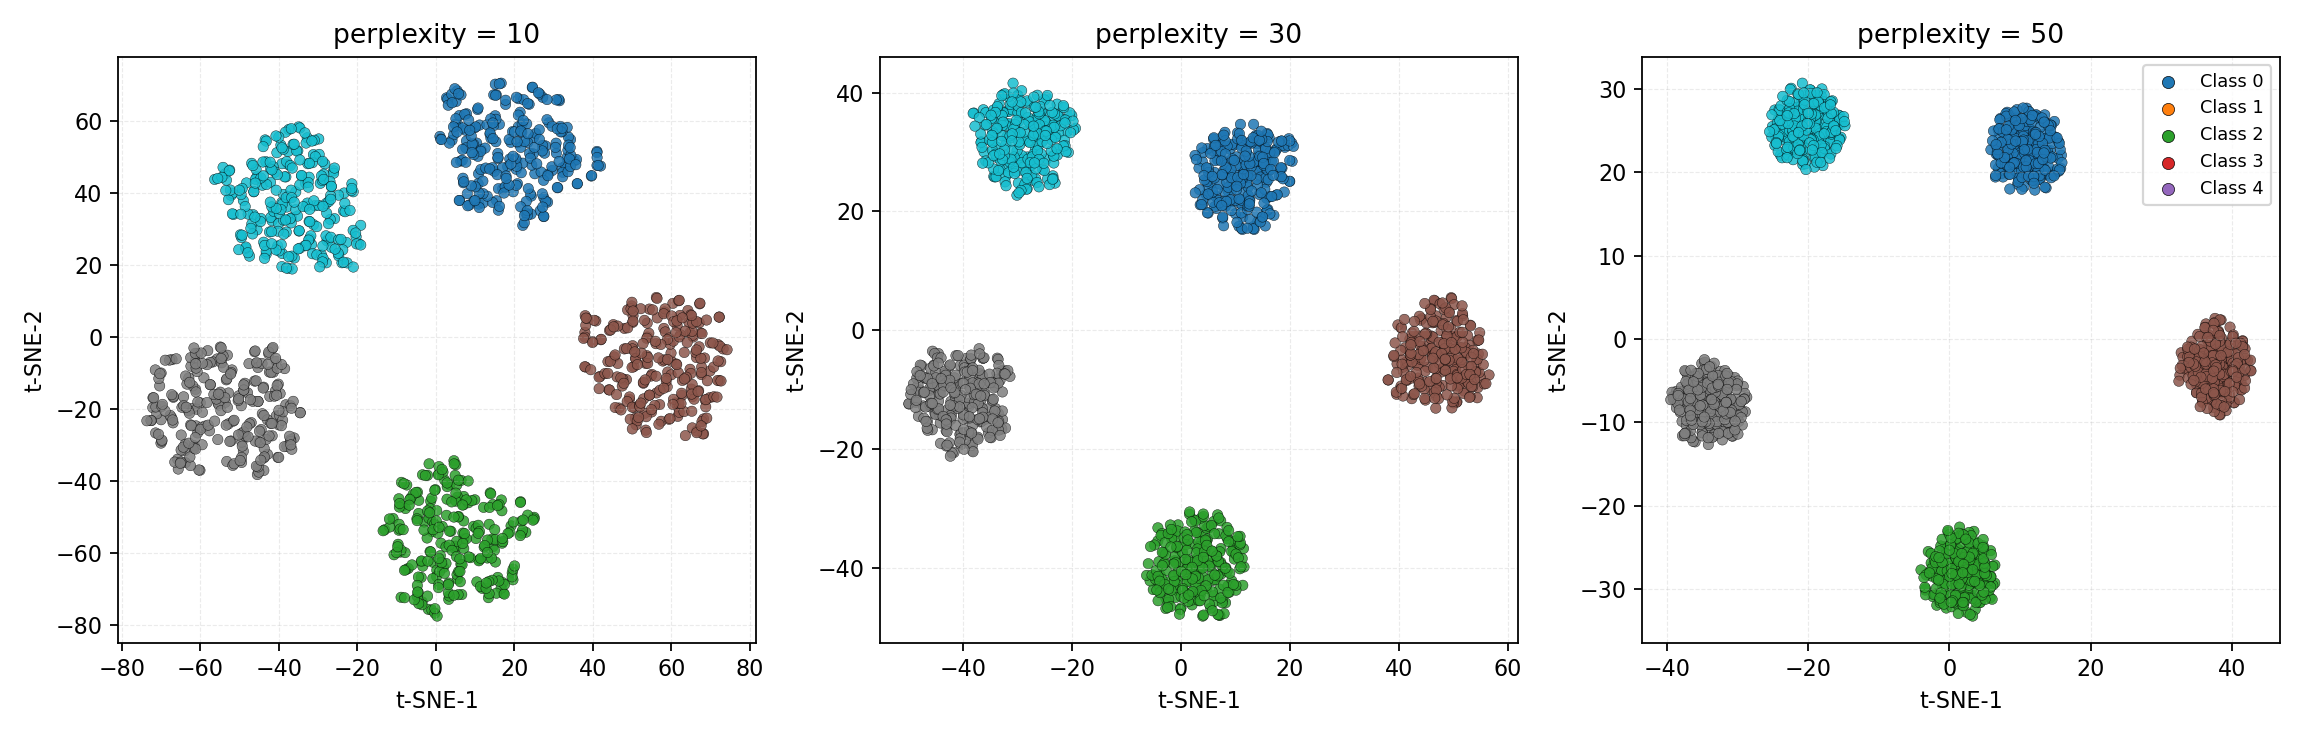
\includegraphics[width=0.82\linewidth]{tsne_embeddings.png}
  \caption{t-SNE embeddings at selected perplexities with coloring by class label}
  \label{fig:tsne_embeddings}
\end{figure}

\begin{figure}[H]
  \centering
  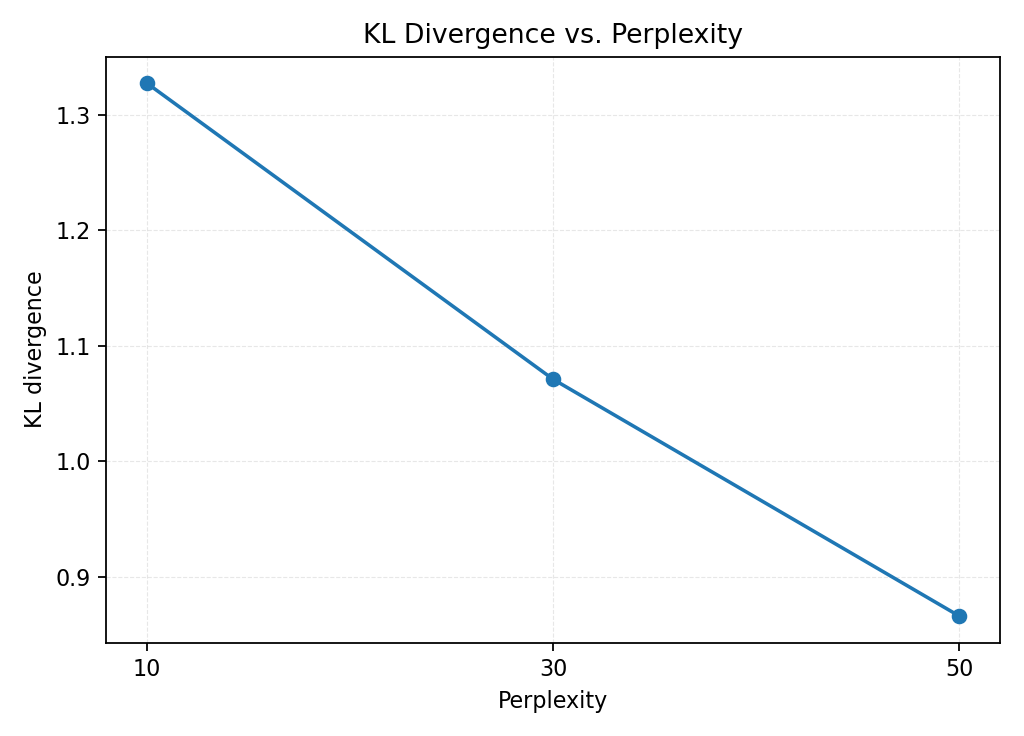
\includegraphics[width=0.8\linewidth]{tsne_perplexity_curve.png}
  \caption{KL divergence versus perplexity illustrating stability ranges}
  \label{fig:tsne_perplexity_curve}
\end{figure}

\FloatBarrier
\section{Summary}
t-SNE captures local neighborhood structure via probabilistic similarity matching and visualizes high-dimensional data with minimal crowding artifacts. Careful tuning of perplexity, learning rate, and iterations yields stable maps that guide exploratory analysis. The example demonstrates how to compare embeddings across perplexities and interpret KL divergence diagnostics.

\end{document}
